% ====================================================================
%+
% SECTION:
%    section-name.tex  % eg lenstimedelays.tex
%
% CHAPTER:
%    chapter.tex  % eg cosmology.tex
%
% ELEVATOR PITCH:
%    Explain in a few sentences what the relevant discovery or
%    measurement is going to be discussed, and what will be important
%    about it. This is for the browsing reader to get a quick feel
%    for what this section is about.
%
% COMMENTS:
%
%
% BUGS:
%
%
% AUTHORS:
%    Phil Marshall (@drphilmarshall)  - put your name and GitHub username here!
%-
% ====================================================================

\section{Disc Intrinsic AGN Variability}
\def\secname{\chpname:variability}\label{sec:\secname}

\credit{ohadshemmer},
\credit{AstroVPK},
{\it Robert Wagoner, and others to follow}

% This individual section will need to describe the particular
% discoveries and measurements that are being targeted in this section's
% science case. It will be helpful to think of a ``science case" as a
% ``science project" that the authors {\it actually plan to do}. Then,
% the sections can follow the tried and tested format of an observing
% proposal: a brief description of the investigation, with references,
% followed by a technical feasibility piece. This latter part will need
% to be quantified using the MAF framework, via a set of metrics that
% need to be computed for any given observing strategy to quantify its
% impact on the described science case. Ideally, these metrics would be
% combined in a well-motivated figure of merit. The section can conclude
% with a discussion of any risks that have been identified, and how
% these could be mitigated.

% A short preamble goes here. What's the context for this science
% project? Where does it fit in the big picture?

A variety of AGN variability studies will be enabled by LSST. These are
intended to probe the physical properties of the unresolved inner regions
of the central engine. Relations will be sought between variability amplitude
and timescale vs. $L$, $z$, $\lambda_{\rm eff}$, color, multiwavelength and
spectroscopic properties, if available. For example, LSST AGNs exhibiting excess
variability over that expected from their luminosities will be further scrutinized
as candidates for lensed systems having unresolved images with the excess
(extrinsic) variability being attributed mainly to microlensing.

Measuring time-delayed responses between variations in the continuum flux
in one LSST band to the continuum flux in another, will be one of the
main themes of AGN science in the LSST era (e.g., \citet{Chelouche2013};
\citet{CheloucheandZucker2013}; \citet{EdelsonEtal2015}; \citet{FausnaughEtal2015}).
Such measurements can test accretion disk models in a robust manner
for a considerably larger number of AGNs than is currently feasible
with microlensing (see section~\ref{sec:microlensing}).

Theories of the hierarchical merger of dark matter halos over cosmic 
time predict that galaxy-galaxy mergers should result in the formation
of a large number of binary SMBHs. This population is predicted to be a strong,
stochastic contributor to the overall gravitational wave background
\citep{2015arXiv151105564T}. The inspiral of gravitationally bound pairs of
SMBHs formed by a major merger may `stall', reducing the gravitational wave
signal \citep{2014SSRv..183..189C}. Potentially periodic AGN variability,
leading to tentative discoveries of binary SMBHs (e.g.,
\citet{2015Natur.525..351D}; \citet{GrahamEtal2015}; \citet{LiuEtal2015}),
may be feasible for LSST for periods ranging from a few
days up to $\sim3$~yr over the entire survey. The fraction of close SMBHs,
tentatively detected by LSST, may provide strong constraints on the strength
of the graviational wave signal expected from the inspiral.

In the deep-drilling fields (DDFs), the LSST sampling is expected to provide
high-quality power spectral density (PSD) functions for $\approx10^{5} - 10^{6}$
AGNs cross $L$, $z$, and $\lambda_{\rm eff}$ down to frequencies of $\sim1$~d$^{-1}$.
These PSDs can enhance AGN selection, and can be used to constrain the SMBH
mass and accretion rate/mode, as well as enable searching for periodic or
quasi-periodic oscillations (QPOs).
%
%Potentially periodic AGN variability, leading to tentative discoveries
%of binary SMBHs (e.g., \citet{GrahamEtal2015}), may also be
%measurable.
%

%Photometric reverberation mapping (PRM), measuring the time-delayed
%response of either the flux of the broad emission line region (BELR)
%lines to the flux of the AGN continuum or between the continuum flux
%in one (longer wavelength) band to the continuum flux in another (band
%with shorter wavelength), will be one of the cornerstones of AGN
%research in the LSST era (e.g., \citet{Chelouche2013};
%\citet{CheloucheandZucker2013}; \citet{CheloucheEtal2014};
%\citet{EdelsonEtal2015}; \citet{FausnaughEtal2015}). For example, LSST
%is expected to deliver BELR line-continuum time delays in
%$\sim10^5-10^6$ sources, which is unprecedented when compared to
%$\sim50-100$ such measurements conducted via the traditional, yet much
%more expensive (per source) spectroscopic method. Sources in the
%deep-drilling fields (DDFs) will benefit from the highest quality PRM
%time-delay measurements given the factor of $\sim10$ denser sampling.


The high-frequency QPO (HFQPO) periods expected from the inner accretion disk
(which provide stable clocks located closer to the horizon as the BH spin increases)
can be estimated from those of the fundamental $g$-mode, which agree with
the observed HFQPO frequencies in stellar-mass BH binaries. Utilizing the
theoretical upper bounds for BH spin and $L/L_{\rm Edd}$, and the lower
bound to the $k$- and bolometric correction $B_n(z)$, one obtains
$\log P({\rm hr}) > 0.4(1-m_n) + \log[(1+z)D_{\rm L}(z)^2]$ for magnitude
$m_n$ in a particular band $n$ and luminosity distance $D_{\rm L}(z)$.
The $k$- and bolometric correction $B_n(z)$ is a decreasing function of BH mass,
but an increasing function of BH spin. The Lyman-alpha forest limits the redshift
range to $z < 2.7$ for $g$-band observations. The HFQPOs will be weaker within longer
wavelength bands.
%The $\sim 80$ visits in the $g$-band proposed for the main survey appears 
%insufficient to produce a useful PSD. The expected HFQPO periods are longer than a few hour visit in a DDF.
For instance, for $m_g  <  23$ and the optimal $z =  2.7$, the HFQPO period is $P > 4$~hr.
%
%QPO search will be most relevant for the DDFs,
Searching for HFQPOs in the DDFs will be most effective if the sampling frequency
in those fields for the $u$ and $g$ bands is at least nightly, i.e., $\gtsim3000$
visits, per band, during the entire survey. Using HFQPOs at such frequencies, LSST will be
sensistive to probing SMBHs down to $\approx10^{5} - 10^{6}~M_{\sun}$. 

%In addition, there's a need for an "ultradeep" field, e.g., the MCs, that will
%be monitored, during commissioning phase, with frequencies in the range ~$1$-$10^4$ min. (i.e., from
%minutes to weeks/months).

% --------------------------------------------------------------------

\subsection{Target measurements and discoveries}
\label{sec:\secname:targets}

%We will measure the power spectral density (PSD) of AGN light 
%curves across $L$, $z$, and $\lambda_{\rm eff}$. Specifically, we will
%measure the short timescale ($\leq 5$~d) spectral index of the PSD and
%the locations of `features' such as QPOs
%and breaks in the PSD.

In the main survey, standard time-series analyses techniques will be used
for measuring time delays between pairs of continuum bands and for detecting
periodic AGNs. Correlation analyses will search for relations between AGN
variability properties and their basic physical parameters. In the DDFs,
such analyses will enable probing deeper and more frequently, resulting in
higher-quality data that will provide stronger constraints from correlation
analyses; the only drawback is the relatively smaller number of sources
available at the high-luminosity end.

A key measurement enabled by the DDFs is a high-quality PSD, in six bands,
for the largest number of AGNs to date. These PSDs, which are rich
in diagnostic power, will be used to search for `features' such as QPOs
and breaks, as well as power-law slopes, that can help constrain SMBH masses
and accretion rates. Additionally, the PSDs can serve as selection
tools, to more effectively distinguish AGNs from variable stars, as
well as a means to propose cadence perturbations to further enhance
AGN selection.

A high-quality PSD, extended to high frequencies, can effectively distinguish
AGNs from other variable sources, assuming AGN light curves are described by
a particular continuous-time autoregressive moving average model (C-ARMA;
\citet{KellyEtal2014}), i.e., C-ARMA(2,1), corresponding to a damped harmonic
oscillator.
%
Determination of the parameters that describe the PSD requires light curve
sampling at least as frequent as $\sim1$~d$^{-1}$. Figure~\ref{PSDvsFreq} shows
the frequency dependence of the spectral index of the PSD for one particular AGN, 
Zw 229-15, observed with {\em Kepler}. The light curve of this source is
well-described by a C-ARMA(2,1) model. The C-ARMA(2,1) model is a higher order
random walk than the damped random walk (DRW) model of \citet{Kelly09}, which
corresponds to a C-ARMA(1,0) model. Recent variability studies indicate that
the simple C-ARMA(1,0) model is insufficient to model AGN variability because
the spectral index of its PSD is mathematically constrained to be 2
\citep{Kelly14,Kasliwal15,Simm15}. Insufficient sampling of an AGN light
curve (e.g., a few times a month), can therefore result in the erroneous conclusion
that a DRW model adequately characterizes the variability.


\begin{figure}
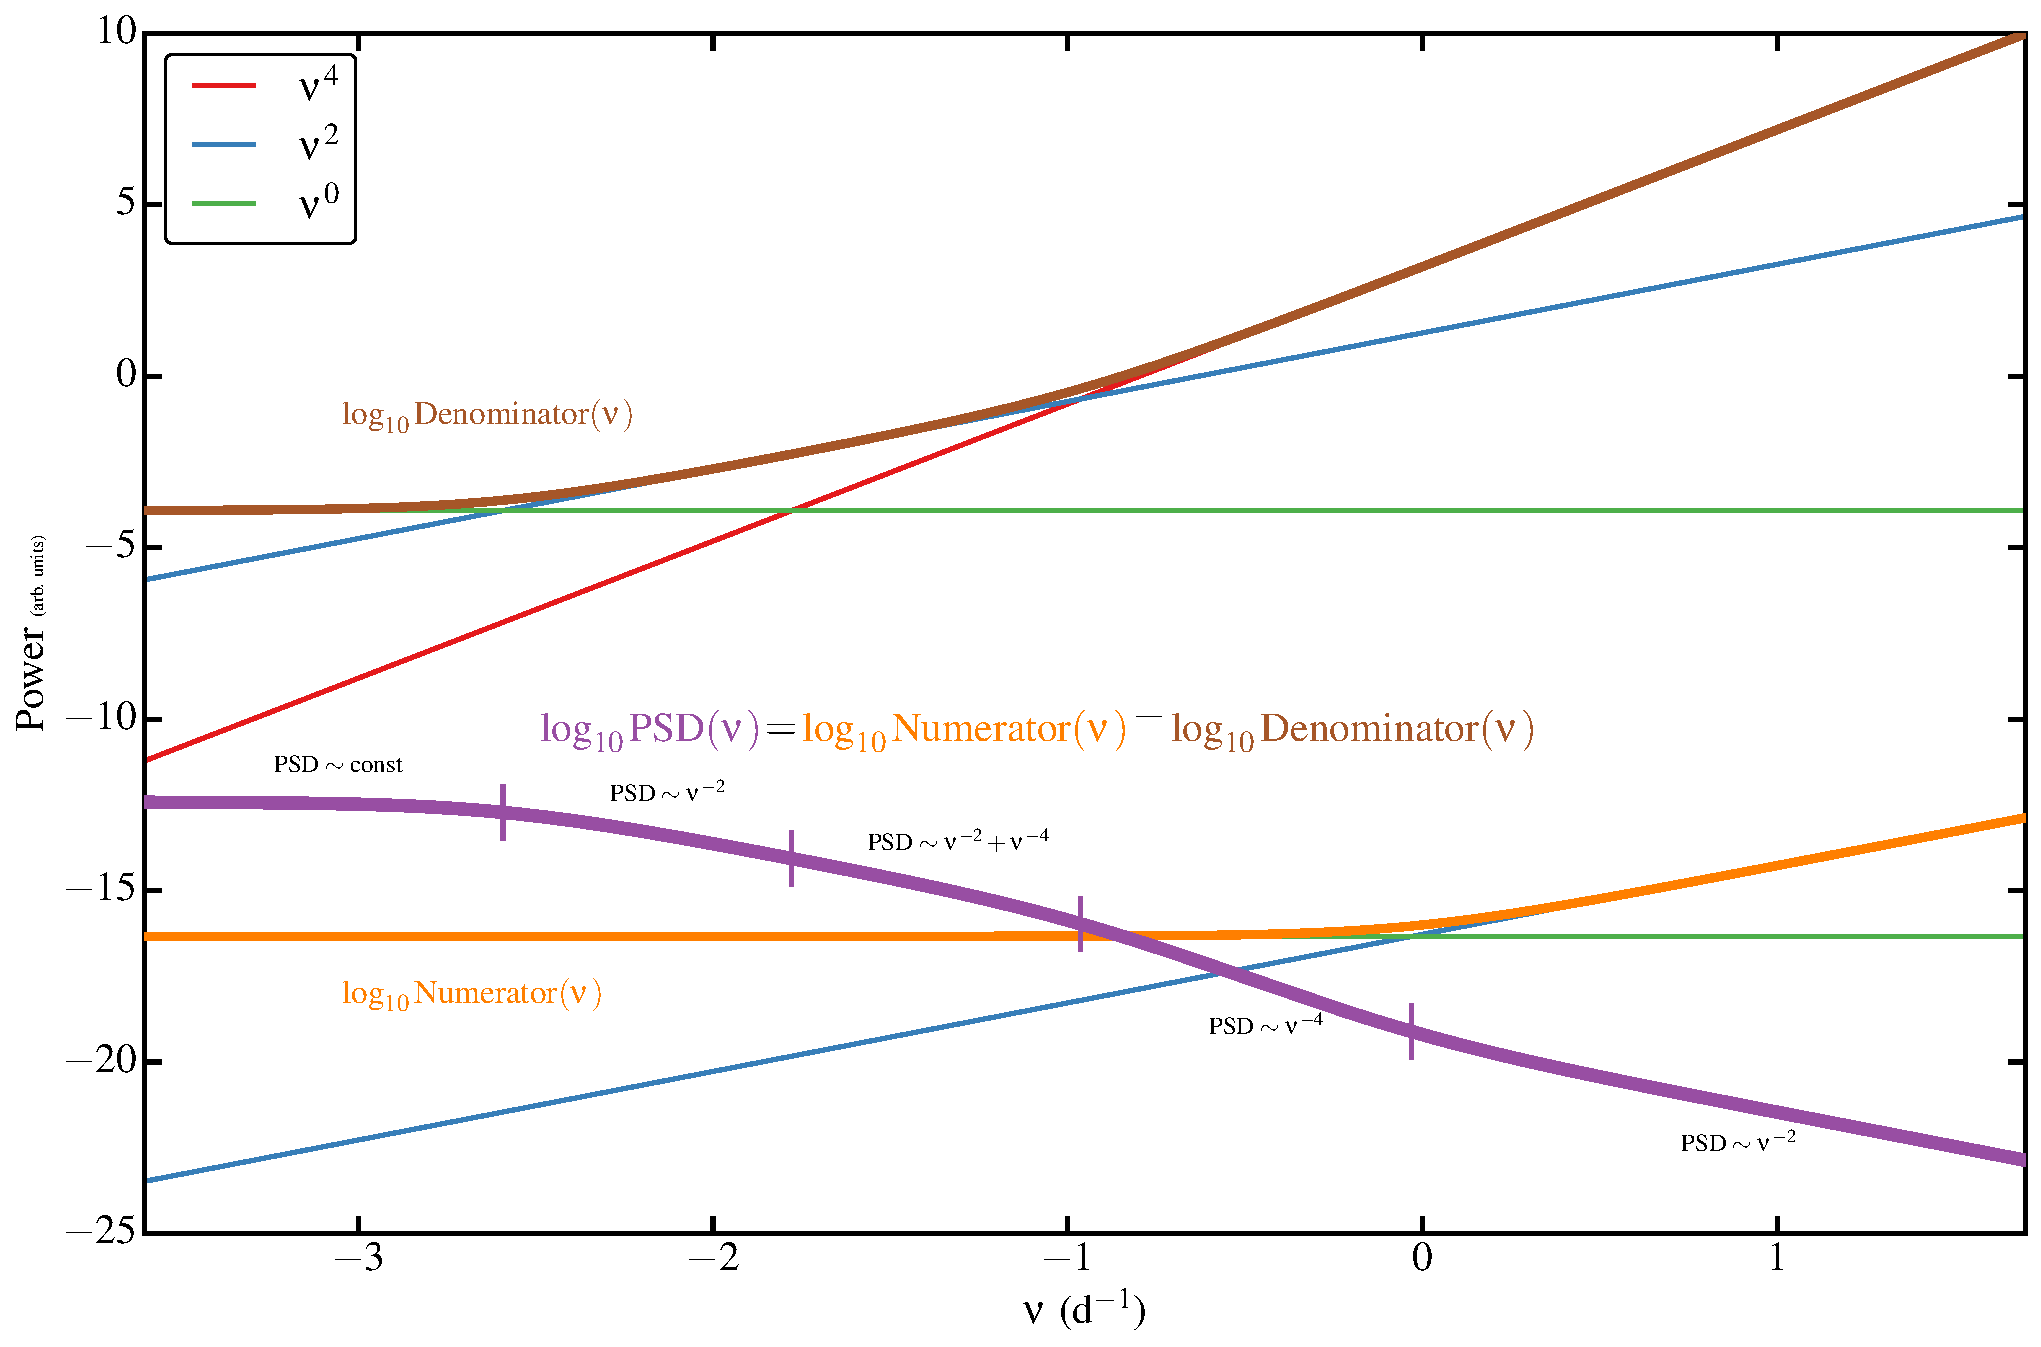
\includegraphics[width=5.0in]{figs/agn/AGN_Variability_01.pdf}
\caption{PSD of Zw 229-15 as a function of frequency, obtained from {\em Kepler}
photometry. The PSD (purple) is the ratio of an even polynomial numerator (orange)
to an even polynomial denominator (brown). This AGN is well-described by a
C-ARMA(2,1) model; different powers of frequency dominate its PSD at different
frequencies depending on the hyperparameters of this model. The wide
frequency range enables detection of PSD spectral index variations ranging
between 0 and 4. Clearly, the light curve of this AGN must be sampled on
timescales {\em shorter} than $1-5$ days in order to observe the $\nu^{-4}$
behavior characteristic of a higher order random walk.
}
\label{PSDvsFreq}
\end{figure}

Accurate recovery of the PSD parameters can be greatly enhanced by increasing the
sampling frequency. To illustrate the effects of the cadence, Figure \ref{CadenceEffect}
shows how the inferred joint distribution of two hyperparameters of the C-ARMA(2,1)
model, the oscillator timescale and the damping ratio, depend on the sampling frequency.
Degrading the sampling frequency from $1/$($30$~min), corresponding to {\em Kepler}
light curves, to $1/$($3$~d), corresponding to the nominal DDF cadence, changes both
the size and the shape of the joint distribution, degrading both the accuracy and
correlation of the inferred hyperparameters.
%
Furthermore, the C-ARMA formalism may enable adjusting the cadence once the LSST survey
begins to determine the sampling pattern in real time.

\begin{figure}
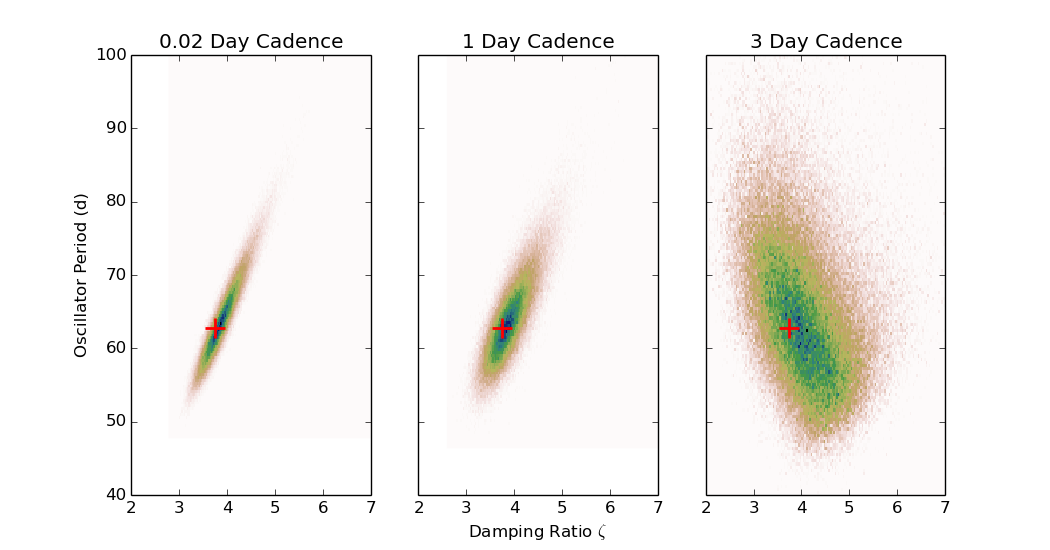
\includegraphics[width=5.0in]{figs/agn/AGN_Variability_00.png}
\caption{The effect of sampling frequency on hyperparameter estimation (courtesy of
J.~Moreno). Light curves were generated using a C-ARMA(2,1) model using the best-fit
parameters for Zw 229-15, observed with {\em Kepler}, indicated by the red cross in
each panel. The light curve was then down-sampled to simulate the effect of observational
cadence. Constraints on the oscillator period and damping ratio begin to widen noticeably
at 3-day sampling. At 1 week and longer cadence (not shown), one does not recover the
correct model order. This strongly indicates the importance of further study to refine
the cadence requirements for LSST.
}
\label{CadenceEffect}
\end{figure}

%The PRM measurements will probe the size and structure of the
%accretion disk and BELR, in a statistical sense, and may provide
%improved SMBH mass estimates for sources that have at least
%single-epoch spectra. \new{Our goal is to understand the population of
%AGN broad line regions, including their geometry. We expect to do this
%via  a model that connects the BH mass, BLR geometry and AGN
%photometric variability properties via a set of scaling relations. A
%simple version of this is could be something like...\newline\newline
%So, our target measurements are of $a$ and $b$, the X parameters.
%Before we derive a metric that quantifies our ability to measure these
%parameters, we can anticipate some of the sensitivity of the
%photometric RM method to observing strategy.}

%\new{We focus on the PSD function as a way of characterizing AGN
%variability in various ways. What do we expect the AGN population to
%look like in PSD parameter space? The hyper-parameters that govern the
%relationships between PSD parameters and  AGN and host galaxy
%properties are probably of greatest scintific interest.}

% --------------------------------------------------------------------

\subsection{Metrics}
\label{sec:\secname:metrics}

Quantifying the response via MAF metrics: definition of the metrics,
and any derived overall figure of merit.

%\new{In lieu of a simulated AGN population, we focus on a few
%particular {\it diagnostic} metrics that capture  our likely ability
%to measure the PSD across the population. These include: the
%uniformity of the sampling pattern in log time lag?}


%Assess the number of meaningful BELR-continuum time delays that can be obtained
%with the nominal OpSim, and point out potential perturbations in the
%cadence to improve the number and quality of such time delays.

While additional work is required for determining the optimal cadence
in order to fully capture AGN accretion physics and to enhance AGN selection,
it is clear that even the nominal DDF sampling is not sufficiently
frequent.

One particular metric for which LSST can make a significant contribution
using the C-ARMA formalism is the selection of low-luminosity AGN (LLAGN),
i.e., sources with $L \ltsim 10^{42}$~erg~s$^{-1}$, in the DDFs. Such
sources are likely to be missed by traditional color-variability selection
algorithms. The metric to be developed should assess how the number of
selected LLAGN depends on the sampling frequency in each band.

% QPOs - Will the cadence and duration give you the proper range on the
% power spectrum to detect QPOs with a given mass, spin, and L/Ledd?
% (Bob Wagoner)

While the ability to detect HFQPOs should also improve by increasing the
sampling frequency, the amplitudes of such features are quite uncertain,
as are the (short) duty cycles. Observations, theory and numerical simulations
have only suggested that the fractional modulation should be small (less than
a few percent). Thus it is not obvious how to choose a metric and observing
strategy to maximize it, other than increasing the sampling frequency to
at least nightly samplings in the $g$ and $u$ bands.

% --------------------------------------------------------------------

\subsection{OpSim Analysis}
\label{sec:\secname:analysis}

OpSim analysis: how good would the default observing strategy be, at
the time of writing for this science project?


% --------------------------------------------------------------------

\subsection{Discussion}
\label{sec:\secname:discussion}

Discussion: what risks have been identified? What suggestions could be
made to improve this science project's figure of merit, and mitigate
the identified risks?

Overall, the key requirement is to increase the nominal sampling frequency
in the DDFs by at least a factor of 3, i.e., having at least 3000 visits,
per band, during the entire survey.

% ====================================================================

\navigationbar
